\interlude[7]{
  Random slides --- The dragon just ate you!
}

% \begin{frame}{Hybrid Security with WireGuard}
% \begin{itemize}
% \item
%   Hybrid post-quantum security due to integration with WireGuard
% \item
%   Session keys produced by Rosenpass used in WireGuard as PSKs
% \item
%   Continuous key renegotiation, every 2 minutes, like WireGuard

%   \begin{itemize}
%   \item
%     When Rosenpass fails to exchange a key, we randomize the WireGuard
%     PSK to make WireGuard fail, too
%   \end{itemize}
% \item
%   This negates some of our advancements in regards to state disruption
%   resistance compared to standalone WireGuard
%
%   \begin{itemize}
%   \item
%     We feel it is worth it though
%   \end{itemize}
% \end{itemize}
% \end{frame}

% \begin{frame}{Rosenpass Usability Goals}
% % :information\_source: (done) Insert infographic kem value naming scheme
% % (sski/spki/\ldots)
% % :information\_source: (done) Insert Infographic ID naming
% % scheme (pidi, sidr)

% % TODO(blipp,marei) fix the layout to something that works
% %                   Questions to Marei: what kind of object is
% %                   a tikzpicture? Why can't I do a newline after one?
%   \begin{columns}[c]
%     \begin{column}{.5\textwidth}

%       \resizebox{.9\textwidth}{!}{%
%         \begin{namepartpicture}
%         \namepart{s=Static,e=Ephemeral}
%         \namepart[3.5cm]{sk=Secret Key,pk=Public Key,pt=Plaintext,ct=Ciphertext}
%         \namepart[7cm]{i=Initiator,r=Responder,m=Mine,t=Theirs}
%         \begin{scope}[decoration={brace,amplitude=5mm},thick]
%         \namebraceright{s}{e}
%         \namebraceleft{sk}{ct}
%         \namebraceright{sk}{ct}
%         \namebraceleft{i}{t}
%         \end{scope}
%         \end{namepartpicture}
%       }

%       \resizebox{.9\textwidth}{!}{%
%         \begin{namepartpicture}
%         \namepart{sid=Session ID, pid=Peer ID}
%         \namepart[3.5cm]{i=Initiator,r=Responder,m=Mine,t=Theirs}
%         \begin{scope}[decoration={brace,amplitude=5mm},thick]
%         \namebraceright{sid}{pid}
%         \namebraceleft{i}{t}
%         \end{scope}
%         \end{namepartpicture}
%       }
%     \end{column}

%     \begin{column}{.5\textwidth}

%       \begin{itemize}
%       \item
%         Focus on being particularly reader-friendly
%       \item
%         Our communication targets non-cryptographers, too
%       \item
%         Somewhat speaking variable names
%       \end{itemize}

%     \end{column}
%   \end{columns}
% \end{frame}

\begin{frame}{Rosenpass and WireGuard: Advanced Security}
\vspace{-\ht\strutbox}
\begin{columns}[fullwidth,T]
  \begin{column}{.49\linewidth}
  \begin{block}{Limited Stealth:\strut}
    \begin{itemize}
      \item Protocol should not respond without pre-auth.
      \item Proof of IP ownership (cookie mechanism) prevents full stealth
      \item Adv. needs to know responder public key
    \end{itemize}
    \end{block}

    \begin{block}{Limited Identity Hiding:\strut}
    \begin{itemize}
      \item Adversary cannot recognize peers unless their public key is known
      \item This is incomplete!
    \end{itemize}
    \end{block}
    % TODO(blipp,karo) why can the adversary not produce a proof?
    %   -- Because the recipient public key could be known by anyone -- karo
  \end{column}

  \begin{column}{.49\linewidth}
    \begin{block}{CPU DoS mitigation:\strut}
    % TODO(blipp,karo) why is it limited? 
    %  -- Because an attacker who knows the public keys can still cause 
    \begin{itemize}
      \item Attacker should not easily trigger public key operations
      \item Preventing CPU exhaustion using network amplification
      \item Proof of IP ownership
    \end{itemize}
    \end{block}

    % \textbf{Interruption resistance:} \vspace{0.5em} % TODO(blipp): Mark red somehow?
    % \begin{itemize}
    %   \item Replay protection based on counters
    %   \item Attacks exist in WireGuard
    %   \item Explicit modeling \& security is a goal in Rosenpass
    % \end{itemize}
    % TODO(blipp,karo) decide how to format the tradeoffs line
    %\item
    %  =\textgreater{} These properties are tradeoffs
  \end{column}
\end{columns}
\end{frame}

% \begin{frame}{Rosenpass Security Properties}

% % TODO(blipp) Make this look more balanced
% % TODO(marei) can the items start further on the left, i.e., no padding on the left?
% % TODO(marei) if this does not solve the space problem, what else could we do to make "Post-Quantum Security" fit into one line in the first column, and the footnote marks in columns 2 and 3?
% % TODO(marei) colors green and red for checkmark and cross?
% % :information\_source: (done) Formosa Retreat slides, slide 2
% \vspace{0.5em}
% \begin{columns}[t]
% \begin{column}{.33\textwidth}
% \heading{WireGuard}
% \begin{itemize}
%   \itemtick Session-key secrecy
%   \itemtick \dots
%   \itemtick Identity Hiding
%   \itemfail \textbf{Non-Interruptability} \footnote[frame]{Assuming a trusted system time}
%   \itemfail \textbf{Post-Quantum Security}
% \end{itemize}
% \end{column}

% \begin{column}{.33\textwidth}
% \heading{
%   PQ WireGuard
%   \footnote[frame]{
% 	  Hülsing, Ning, Schwabe, Weber, Zimmermann. “Post-quantum WireGuard”. https://ia.cr/2020/379
% 	}
% }
% \begin{itemize}
%   \itemtick \textbf{Post-Quantum Security}
%   \itemfail \textbf{Hybrid security}
%   \itemfail \textbf{Non-Interruptability} \footnote[frame]{Assuming a PSK}
% \end{itemize}
% \end{column}

% \begin{column}{.33\textwidth}
% \heading{Rosenpass}
% \begin{itemize}
%   \itemtick \textbf{Non-Interruptability} \footnote[frame]{Through cookies}
%   \itemtick \textbf{Hybrid security} \footnote[frame]{Used together with standard WireGuard}
% \end{itemize}
% \end{column}

% \end{columns}
% \vspace{1.5em}

% \end{frame}

%TODO(marei) Can this code be better/more LaTeX-y?
\interlude[1]<Triumphs \textasciitilde\ Secrecy \& Non-Interruptability>{Modeling of Rosenpass}<Using ProVerif>

% TODO Blipp: Insert example as discussed
% \begin{frame}{Symbolic modeling: Exposure scenario enumeration}
% \begin{itemize}
%   \item Covers a broad range of exposure scenarious
%   \item Plain listing of minimum conditions for secrecy of the output key to hold
%   \item Modeling of various exposure scenarious such as ephemeral key and both peer keys being the same key
% \end{itemize}
% \end{frame}

\begin{frame}{Non-Interruptability: More Formally}
    For every pair of traces $\mathtt{tmin}, \mathtt{tmax}$ where trace $\mathtt{tmax}$ can be formed by
    insertion of messages/oracle calls into $\mathtt{tmin}$, the result of $\mathtt{tmin}$ and $\mathtt{tmax}$
    should remain the same.

	

    \begin{itemize}
      \item Let $\mathtt{Result}$ be the set of possible protocol results
      \item Let $\mathtt{Trace}$ be the set of possible protocol traces
      \item Let $\mathtt{res}(\mathtt{t}) : \mathtt{Trace} \to \mathtt{Result}$ determine the protocol result given $\mathtt{t} : \mathtt{Trace}$
      \item Let $\mathtt{t1} \supseteq \mathtt{t2} : \mathtt{Trace} \to \mathtt{Trace} \to \mathtt{Prop}$ denote that $\mathtt{t}2$ can be formed by insertion of elements into $\mathtt{t}1$
      \item $\forall (\mathtt{tmin}, \mathtt{tmax}) : \mathtt{Trace} \times \mathtt{Trace}; \mathtt{tmin} \supseteq \mathtt{tmax} \to \mathtt{res}(\mathtt{tmin}) = \mathtt{res}(\mathtt{tmax})$
    \end{itemize}
    \pdfpcnote{Karo}
\end{frame}

% TODO: Blipp. Insert example to explain
% @lemma "non-interruptability: Adv cannot prevent a genuine InitConf message from being accepted"
% lemma ih:InitHello_t, rh:RespHello_t, ic:InitConf_t, psk:key, sski:kem_sk, sskr:kem_sk;
  % event(ICRjct(ic, psk, sskr, kem_pub(sski)))
  % && event(IHSent(ih, psk, sski, kem_pub(sskr)))
  % && event(RHSent(ih, rh, psk, sskr, kem_pub(sski)))
  % && event(ICSent(rh, ic, psk, sski, kem_pub(sskr))).
% \begin{frame}{Symbolic modeling: Non-Interruptability}
% \begin{itemize}
%   \item Non-Interruptability is security from disruption attacks
%   \item 
%   % TODO Blipp: Add more formal definition?
% \end{itemize}
% \end{frame}


% \begin{frame}{Rosenpass Security Analysis}
% % TODO(marei) see line below
% % :information\_source: Insert proverif in technicolor screenshot in
% % the right side. Cut off. Clearly marked as decoration

% \begin{columns}[c]
%     \begin{column}{.5\textwidth}
%       \begin{itemize}
%       \item
%         Symbolic analysis of Secrecy, Authenticity, and MEX attacks in
%         ProVerif

%         \begin{itemize}
%         \item
%           Novel model of different exposure scenarios
%         \item
%           Essentially listing minimum requirements for security properties to
%           hold
%         \end{itemize}
%       \item
%         Symbolic analysis of State Disruption Resistance in ProVerif

%         \begin{itemize}
%         \item
%           Modeled using ``package accept'' and ``package rejected'' events in
%           the protocol transcript
%         \item
%           Adversary's inability to produce a ``package rejected'' event for a
%           valid handshake message
%         \end{itemize}
%       \end{itemize}

%     \end{column}

%     \begin{column}{.5\textwidth}
%       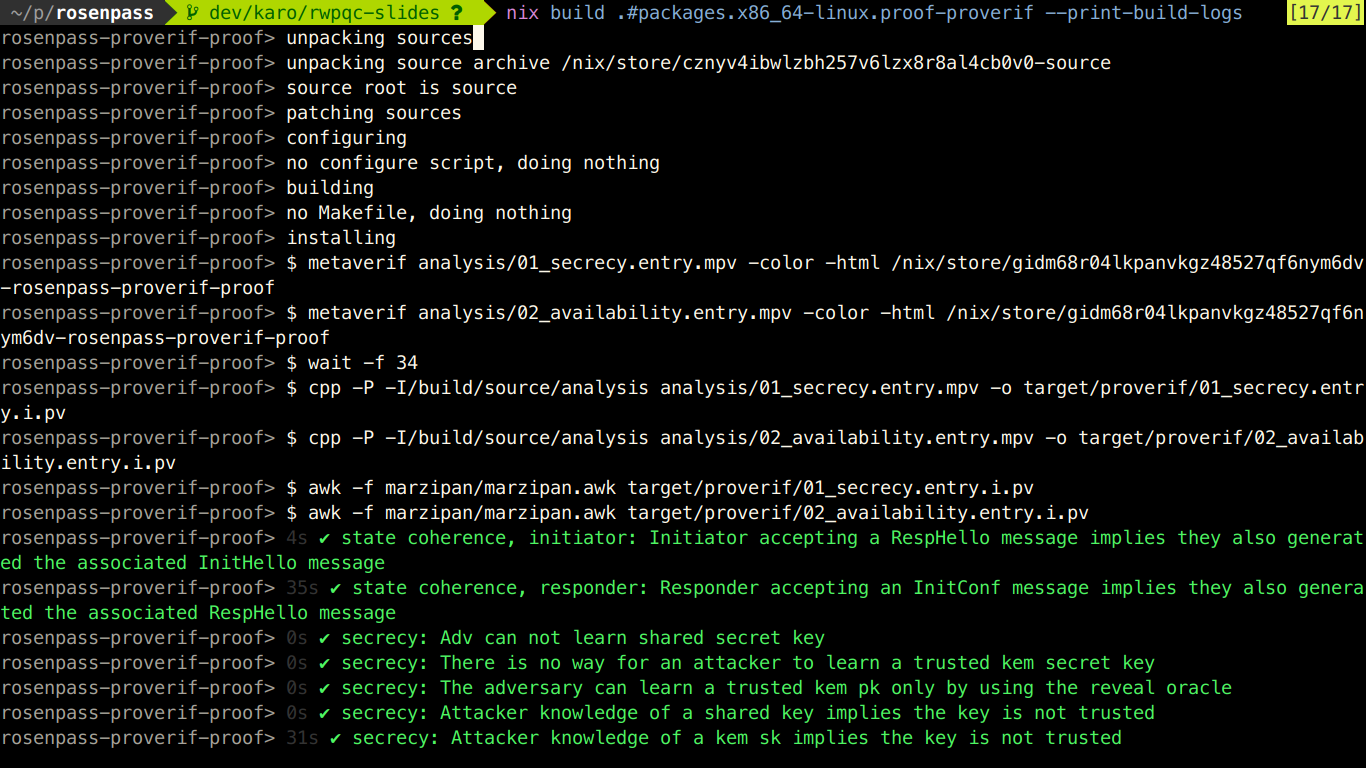
\includegraphics[keepaspectratio,width=.9\textwidth]{2023-03-20-symbolic-analysis-screenshot.png}

%     \end{column}
%   \end{columns}
% \end{frame}

\begin{frame}{ChronoTrigger Attack: Immediate Execution}
\begin{columns}[fullwidth,T]
  \begin{column}{.5\linewidth}
    \rlap{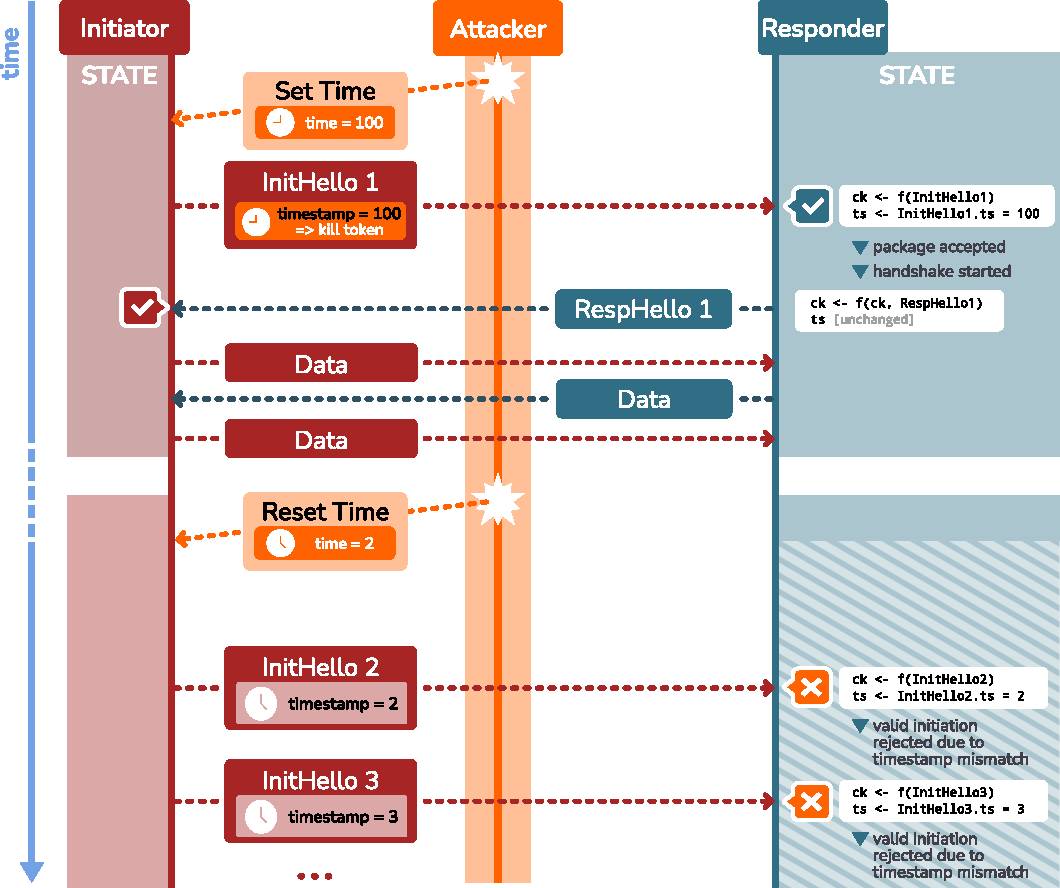
\includegraphics[height=.85\textheight]{graphics/chronotrigger-immediate-bare.pdf}}
  \end{column}

  \begin{column}{.46\linewidth}
    \small\leavevmode
      \begin{enumblock}{Preparation phase:}
      \begin{enumerate}
        \item \textbf{Attacker} sets \emph{initiator system time} to a future value
        \item \textbf{Attacker} waits while both peers are performing a valid handshake
      \end{enumerate}
      \end{enumblock}
      \begin{enumblock}{Direct execution phase:}
      \begin{enumerate}
        \item \textbf{Attacker} lets system time on initiator reset
        \item[=>] Initiation now fails due to counter mismatch
      \end{enumerate}
      \end{enumblock}
  \end{column}
\end{columns}
\end{frame}

\begin{frame}{ChronoTrigger: Changes in Post-Quantum WG}
  \begin{columns}[fullwidth,T]
    \begin{column}{.5\linewidth}
      \rlap{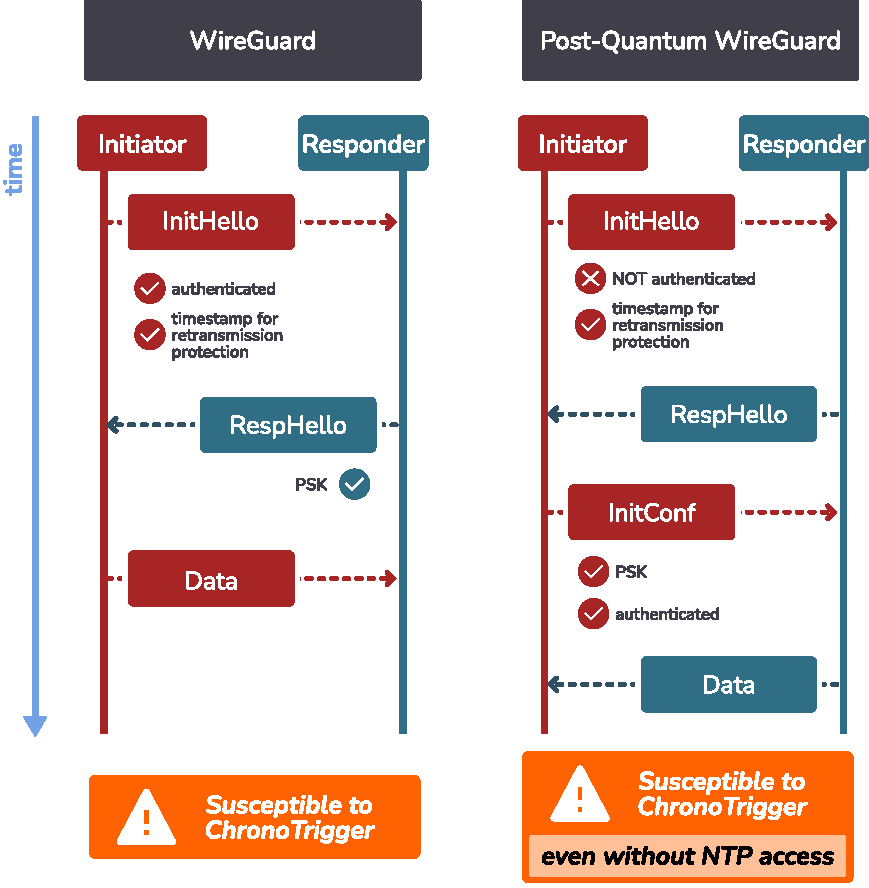
\includegraphics[height=.85\textheight]{graphics/chronotrigger-compare-wg-pqwg.pdf}}
    \end{column}

    \begin{column}{.46\linewidth}
      \begin{itemize}
        \item \emph{InitHello} is unauthenticated
        \item Retransmission counter is kept
        \item PQWG assumes a pre-shared key to authenticate InitHello instead (the authors recommend deriving the PSK from both public keys)
        \item PSK evaluated twice, during InitHello \emph{and} InitConf processing
      \end{itemize}
    \end{column}
  \end{columns}
\end{frame}

\begin{frame}{ChronoTigger against Post-Quantum WireGuard}
  \begin{columns}[fullwidth,T]
    \begin{column}{.5\linewidth}
     \rlap{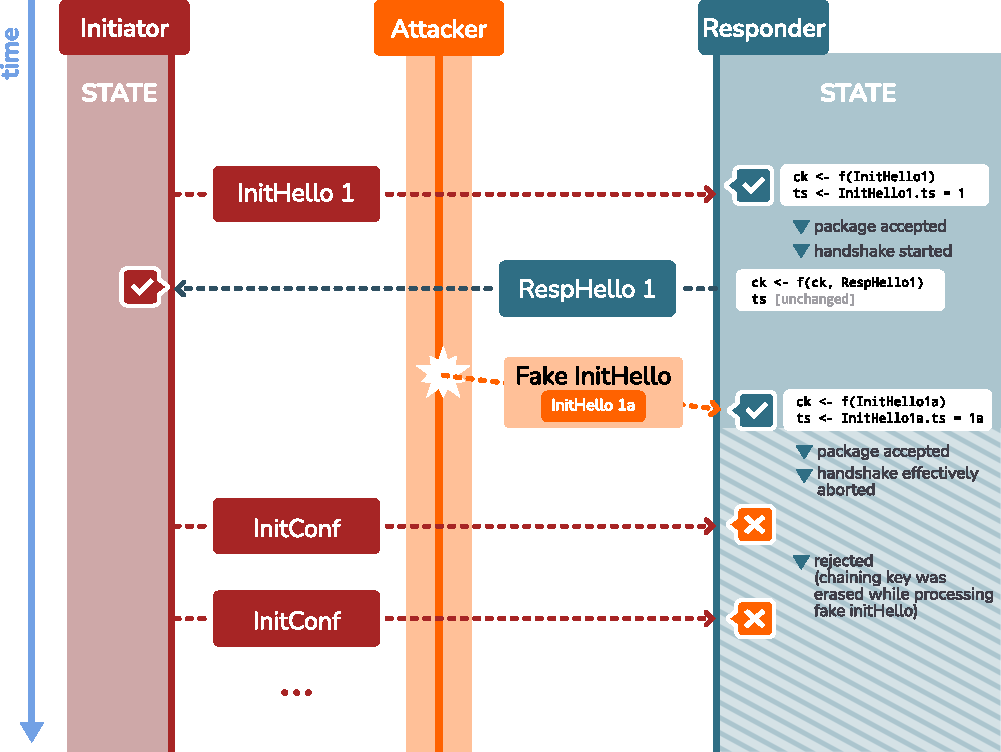
\includegraphics[height=.85\textheight]{graphics/pqwg-state-disrupt-bare.pdf}}
    \end{column}

    \begin{column}{.4\linewidth}
      \begin{block}{No PSK/Public keys as PSK}
      \begin{itemize}
        \item Attacker needs access to public keys
        \item The attack is trivial (attacker just forges \emph{InitHello})
      \end{itemize}
      \end{block}

      \begin{block}{With PSK}
      \begin{itemize}
        \item Replay attack with NTP access from classic WireGuard still applies
      \end{itemize}
      \end{block}
    \end{column}
  \end{columns}
\end{frame}

\interlude[3]<Trials \textasciitilde\ Attacks found>{CookieCutter}

\begin{frame}{CookieCutter Attack}
\only<+|handout:+>{
    \begin{columns}[fullwidth,c]
      \begin{column}{.5\linewidth}
        \blockquote[\textbf{A WireGuard CookieReply}, ca. 2014]{
          I am under load. Prove that you are not using IP address impersonation before I process your handshake! 

          This message contains a \emph{cookie key}. Use it to prove that you can receive messages sent to your
          address when retransmitting your \emph{InitHello} packet.}
      \end{column}

      \begin{column}{.4\linewidth}
        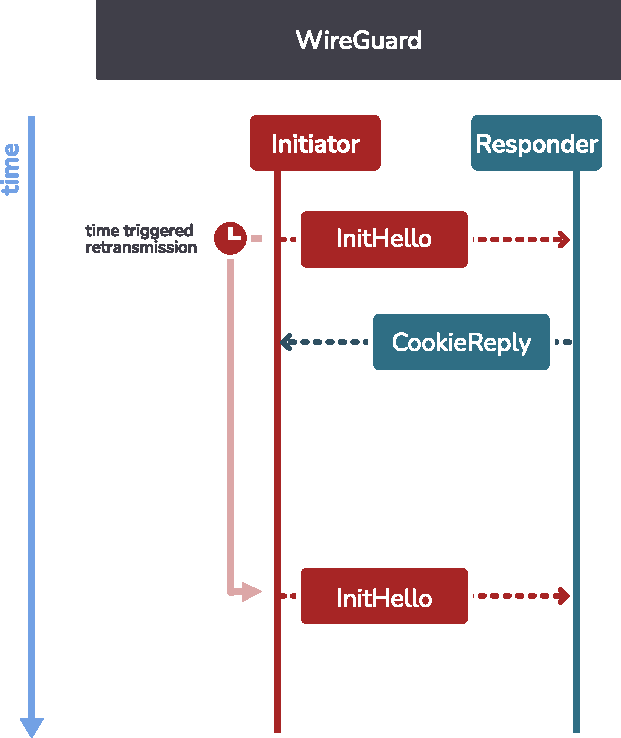
\includegraphics[height=.85\textheight]{graphics/wg-cookiereply.pdf}
      \end{column}
    \end{columns}
  }


    \begin{columns}[fullwidth,T]
      \begin{column}<+-|handout:+->{.4\linewidth}
        % TODO(marei) could we avoid that the picture jumps in its vertical position?
        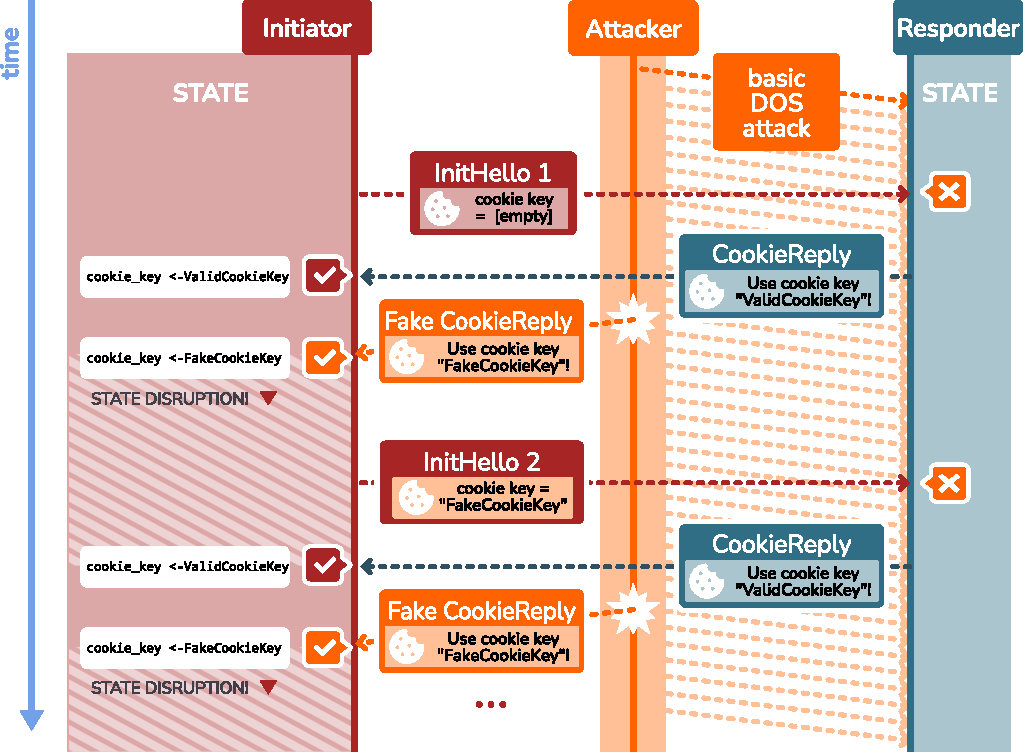
\includegraphics[height=.85\textheight]{graphics/cookiecutter-bare}
      \end{column}
      \begin{column}{.4\linewidth}
      \small
      \only<.|handout:.>{
      	\vspace{-\ht\strutbox}
          \begin{enumerate}
            \item \textbf{Attacker} begins continuous DoS attack against responder
            \item \textbf{Initiator} begins handshake, sends \emph{InitHello}
            \item \textbf{Responder} replies with \emph{CookieReply}
              \blockquote{\textbf{CookieReply:} I am under load. Prove you are not using an IP spoofing attack with this \emph{cookie key}.}
            \item \textbf{Initiator} Initiator stores cookie key and waits for their retransmission timer
            \item \textbf{Attacker} forges a cookie reply with a fake \emph{cookie key}
            \item \textbf{Initiator} Initiator overwrites the valid cookie key with the fake one
            \item[…] Repeat ad nauseam
          \end{enumerate}
      }

        \only<+|handout:+>{%
          \vspace{-\ht\strutbox}\begin{block}{Attacker gains:}
          \begin{itemize}
            \item Cheap protocol-level DoS
          \end{itemize}
          \unskip
          \end{block}
          \begin{block}{Attacker needs:}
          \begin{itemize}
            \item Knowledge of public keys
            \item Good timing 
          \end{itemize}
          \unskip
          \end{block}
          \begin{block}{Role switching:}
          \begin{itemize}
            \item WireGuard sometimes uses role switching
            \item To account for that, the attack can be performed against both peers 
          \end{itemize}
          \unskip
          \end{block}
        }
      \end{column}
    \end{columns}
\end{frame}

\begin{frame}{CookieCutter: Post-Quantum WG \& Rosenpass}
  \begin{columns}[fullwidth,T]
    \begin{column}{.6\linewidth}
      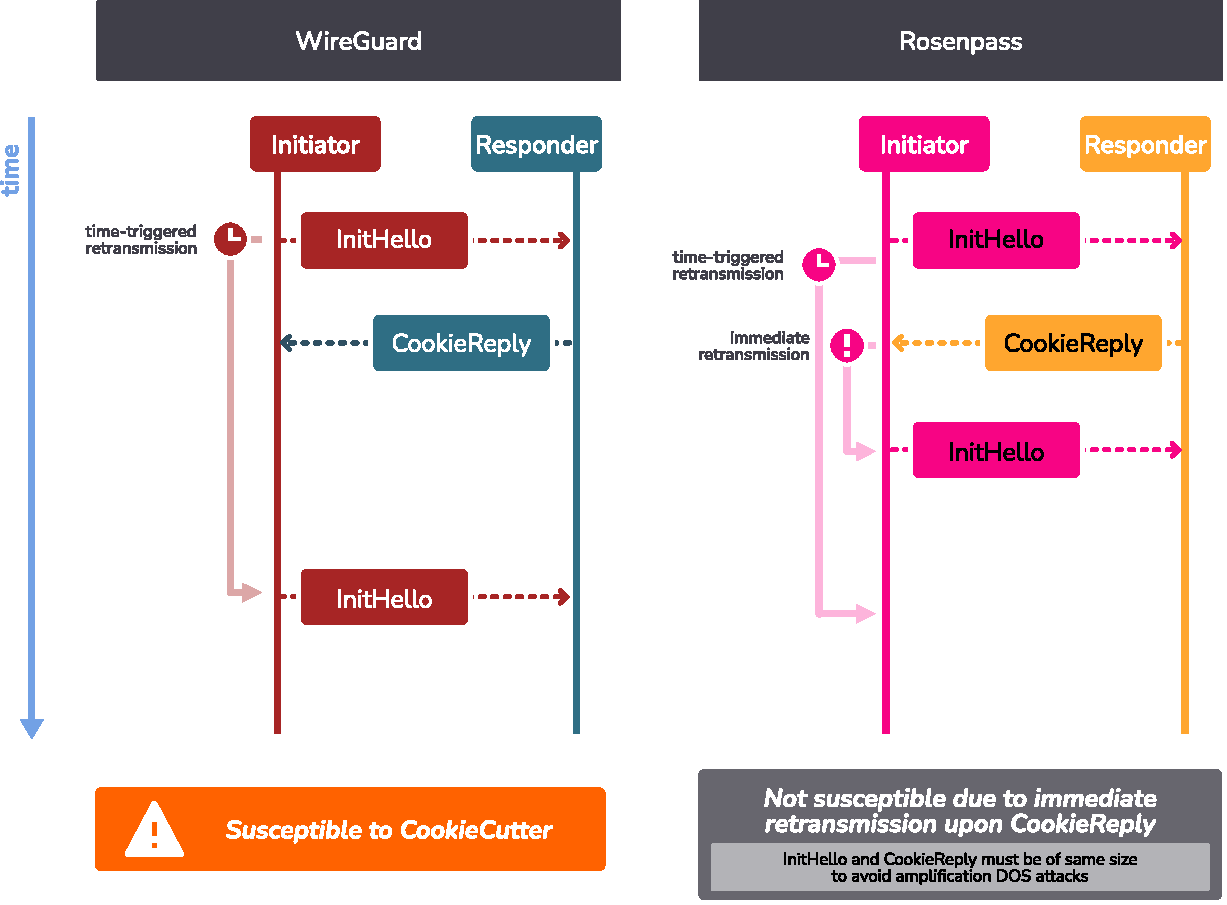
\includegraphics[keepaspectratio,height=.85\textheight]{graphics/cookiecutter-compare.pdf}
    \end{column}

    \begin{column}{.4\linewidth}
      \begin{block}{Post-Quantum WireGuard}
      \begin{itemize}
        \item No change.
      \end{itemize}
      \end{block}

      \begin{block}{Rosenpass}
      \begin{itemize}
        \item Immediate retransmission of \emph{InitHello} upon receiving \emph{CookieReply}
        \item \emph{CookieReply} and \emph{InitHello} must be of same size to prevent DoS amplication attacks
        \item[$\Rightarrow$] Rosenpass is protected from CookieCutter attacks
      \end{itemize}
      \end{block}
    \end{column}
  \end{columns}
\end{frame}

% \begin{frame}{CookieCutter: Post-Quantum WireGuard}
%   \begin{columns}[c]
%     \begin{column}{.4\textwidth}
%       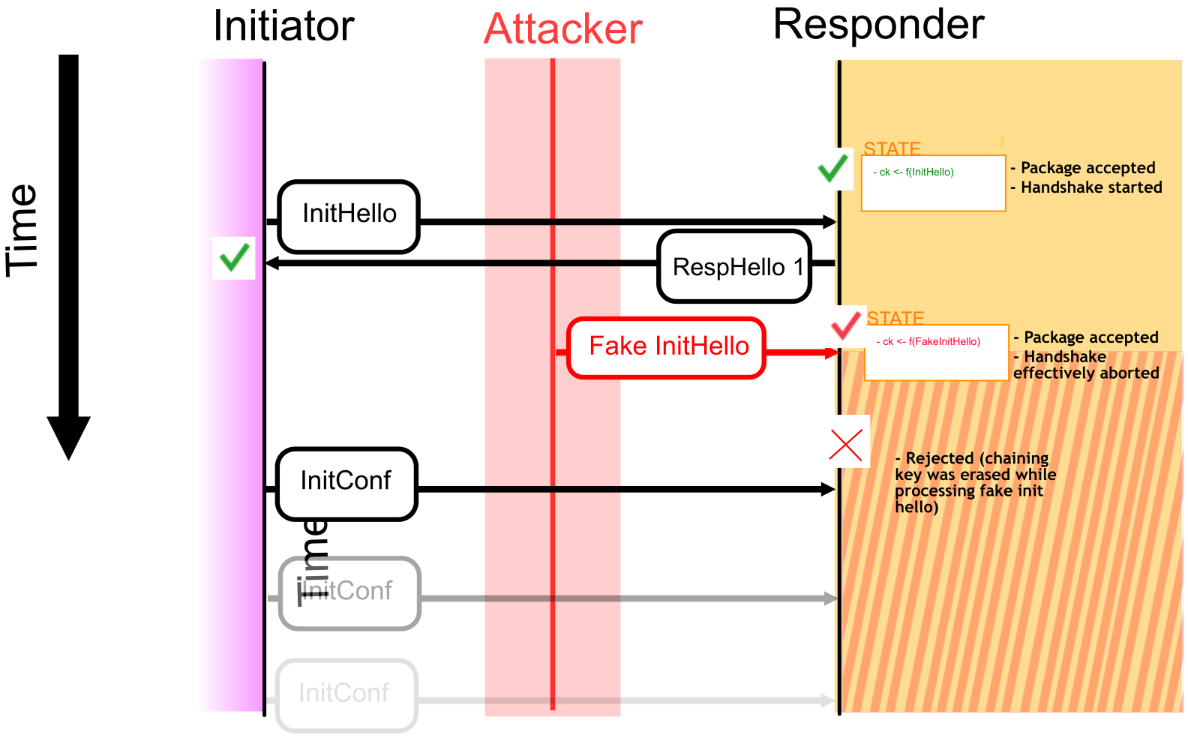
\includegraphics[keepaspectratio,width=.9\textwidth]{graphics/pqwg-state-disrupt.png}
%     \end{column}

%     \begin{column}{.6\textwidth}

%       \begin{itemize}
%       \item
%         State Disruption of Post-Quantum WireGuard is simple forgery
%         \begin{itemize}
%         \item
%           Or replay attack (if public keys are not known)
%         \end{itemize}
%       \item
%         ChronoTrigger attack still works (no NTP access needed if public keys
%         are known)
%       \end{itemize}
%     \end{column}
%   \end{columns}
% \end{frame}

% \begin{frame}{CookieCutter: Post-Quantum WireGuard and Rosenpass}
%   \begin{columns}[c]
%     \begin{column}{.4\textwidth}
%       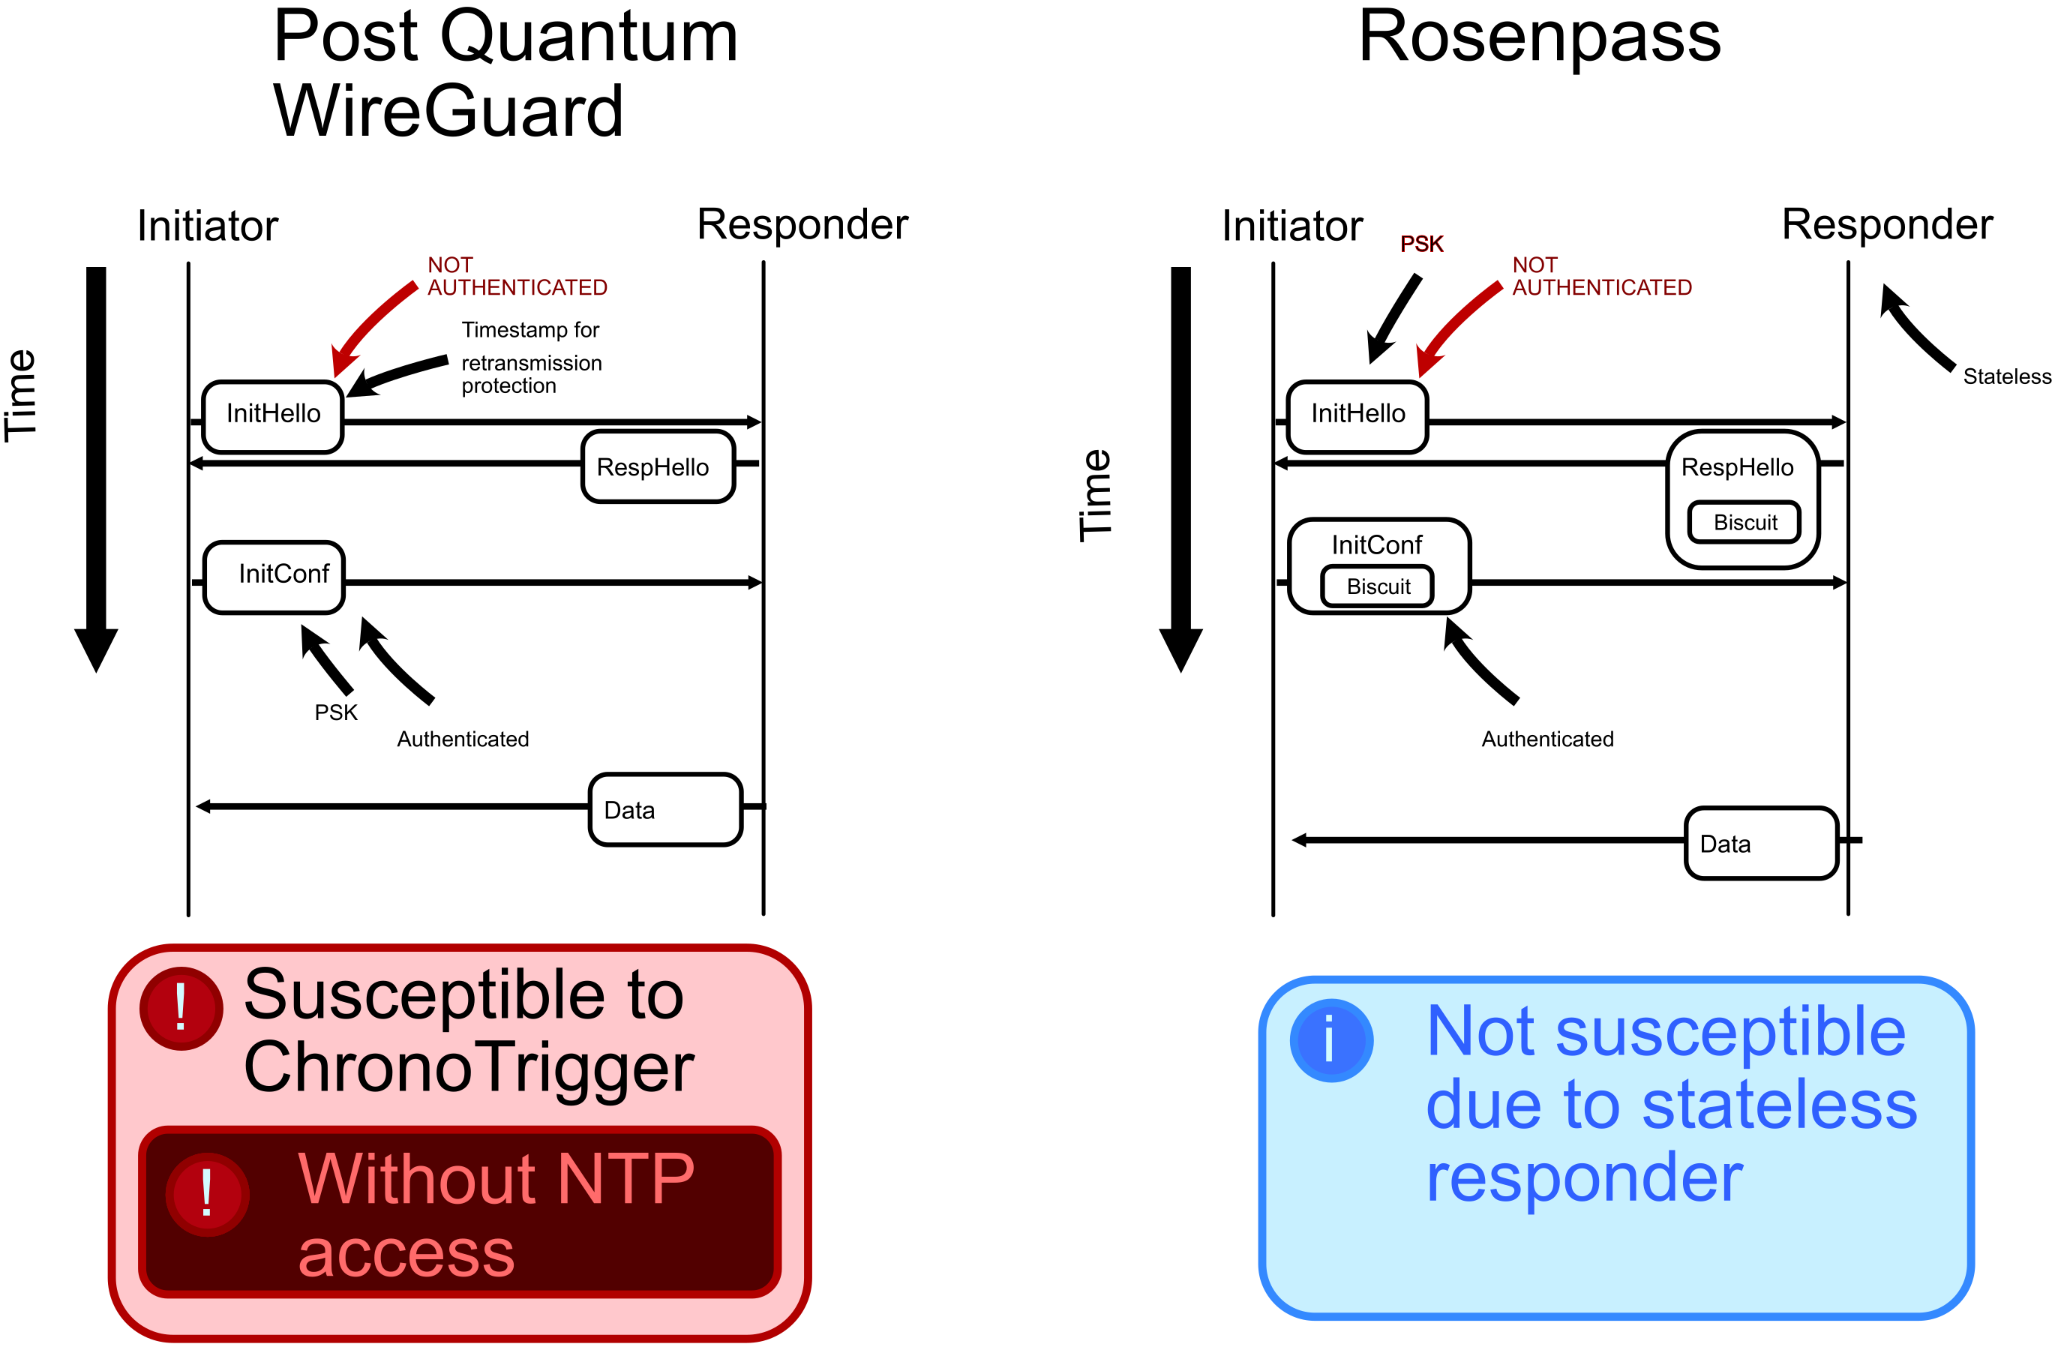
\includegraphics[keepaspectratio,width=.9\textwidth]{graphics/pqwg-rosenpass-compare.png}
%     \end{column}

%     \begin{column}{.6\textwidth}
%       \begin{itemize}
%       \item Moved PSK into (only) InitHello
%       \item
%         Stateless responder to prevent state disruption

%         \begin{itemize}
%         \item
%           State moved into biscuit
%         \end{itemize}
%       \item
%         InitHello immediately retransmitted upon CookieReply reception

%         \begin{itemize}
%         \item
%           CookieReply must be as big as InitHello to avoid amplification
%           attacks
%         \end{itemize}
%       \end{itemize}
%     \end{column}
%   \end{columns}
% \end{frame}


% \begin{frame}{ChronoTrigger Protocol Comparison}
% % :information\_source: (done) Dedicated scientific illustration

% % TODO(marei) see line below
% % :information\_source: Resize illustrations to make room for points

%   \begin{columns}[c]
%     \begin{column}{.4\textwidth}
%       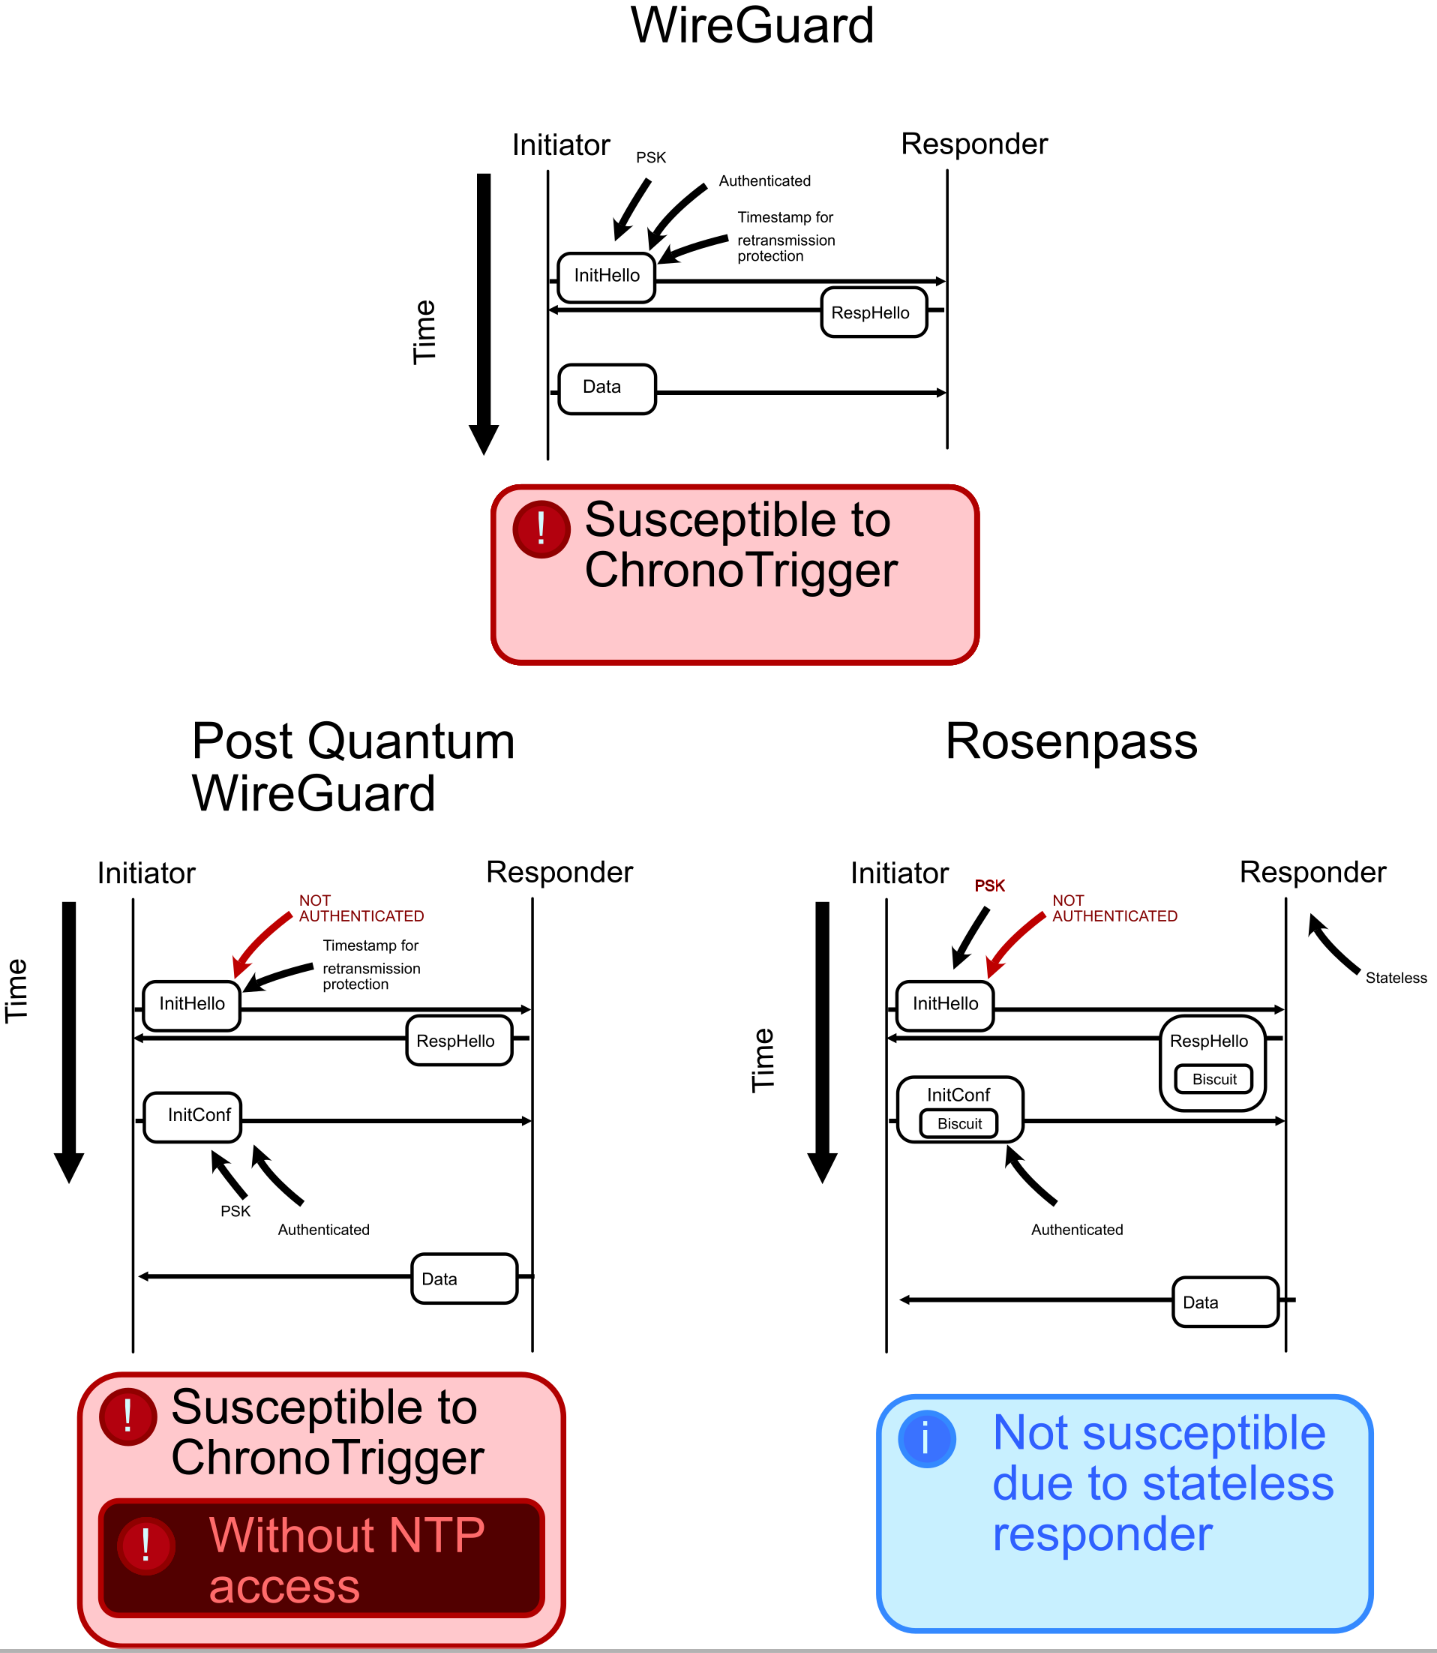
\includegraphics[keepaspectratio,width=.9\textwidth]{graphics/chronotrigger-compare.png}
%     \end{column}

%     \begin{column}{.6\textwidth}
%       \begin{itemize}
%       \item
%         WireGuard: Affected
%       \item
%         Post-Quantum WireGuard: Worse (public key knowledge is sufficient for
%         kill token generation)
%       \item
%         Rosenpass: Secured by being stateless
%       \end{itemize}
%     \end{column}
%   \end{columns}
% \end{frame}

% \begin{frame}{CookieCutter Protocol Comparison}
% % :information\_source: (done) Dedicated scientific illustration

% % TODO(marei) see line below
% % :information\_source: Resize illustrations to make room for points

%   \begin{columns}[c]
%     \begin{column}{.4\textwidth}
%       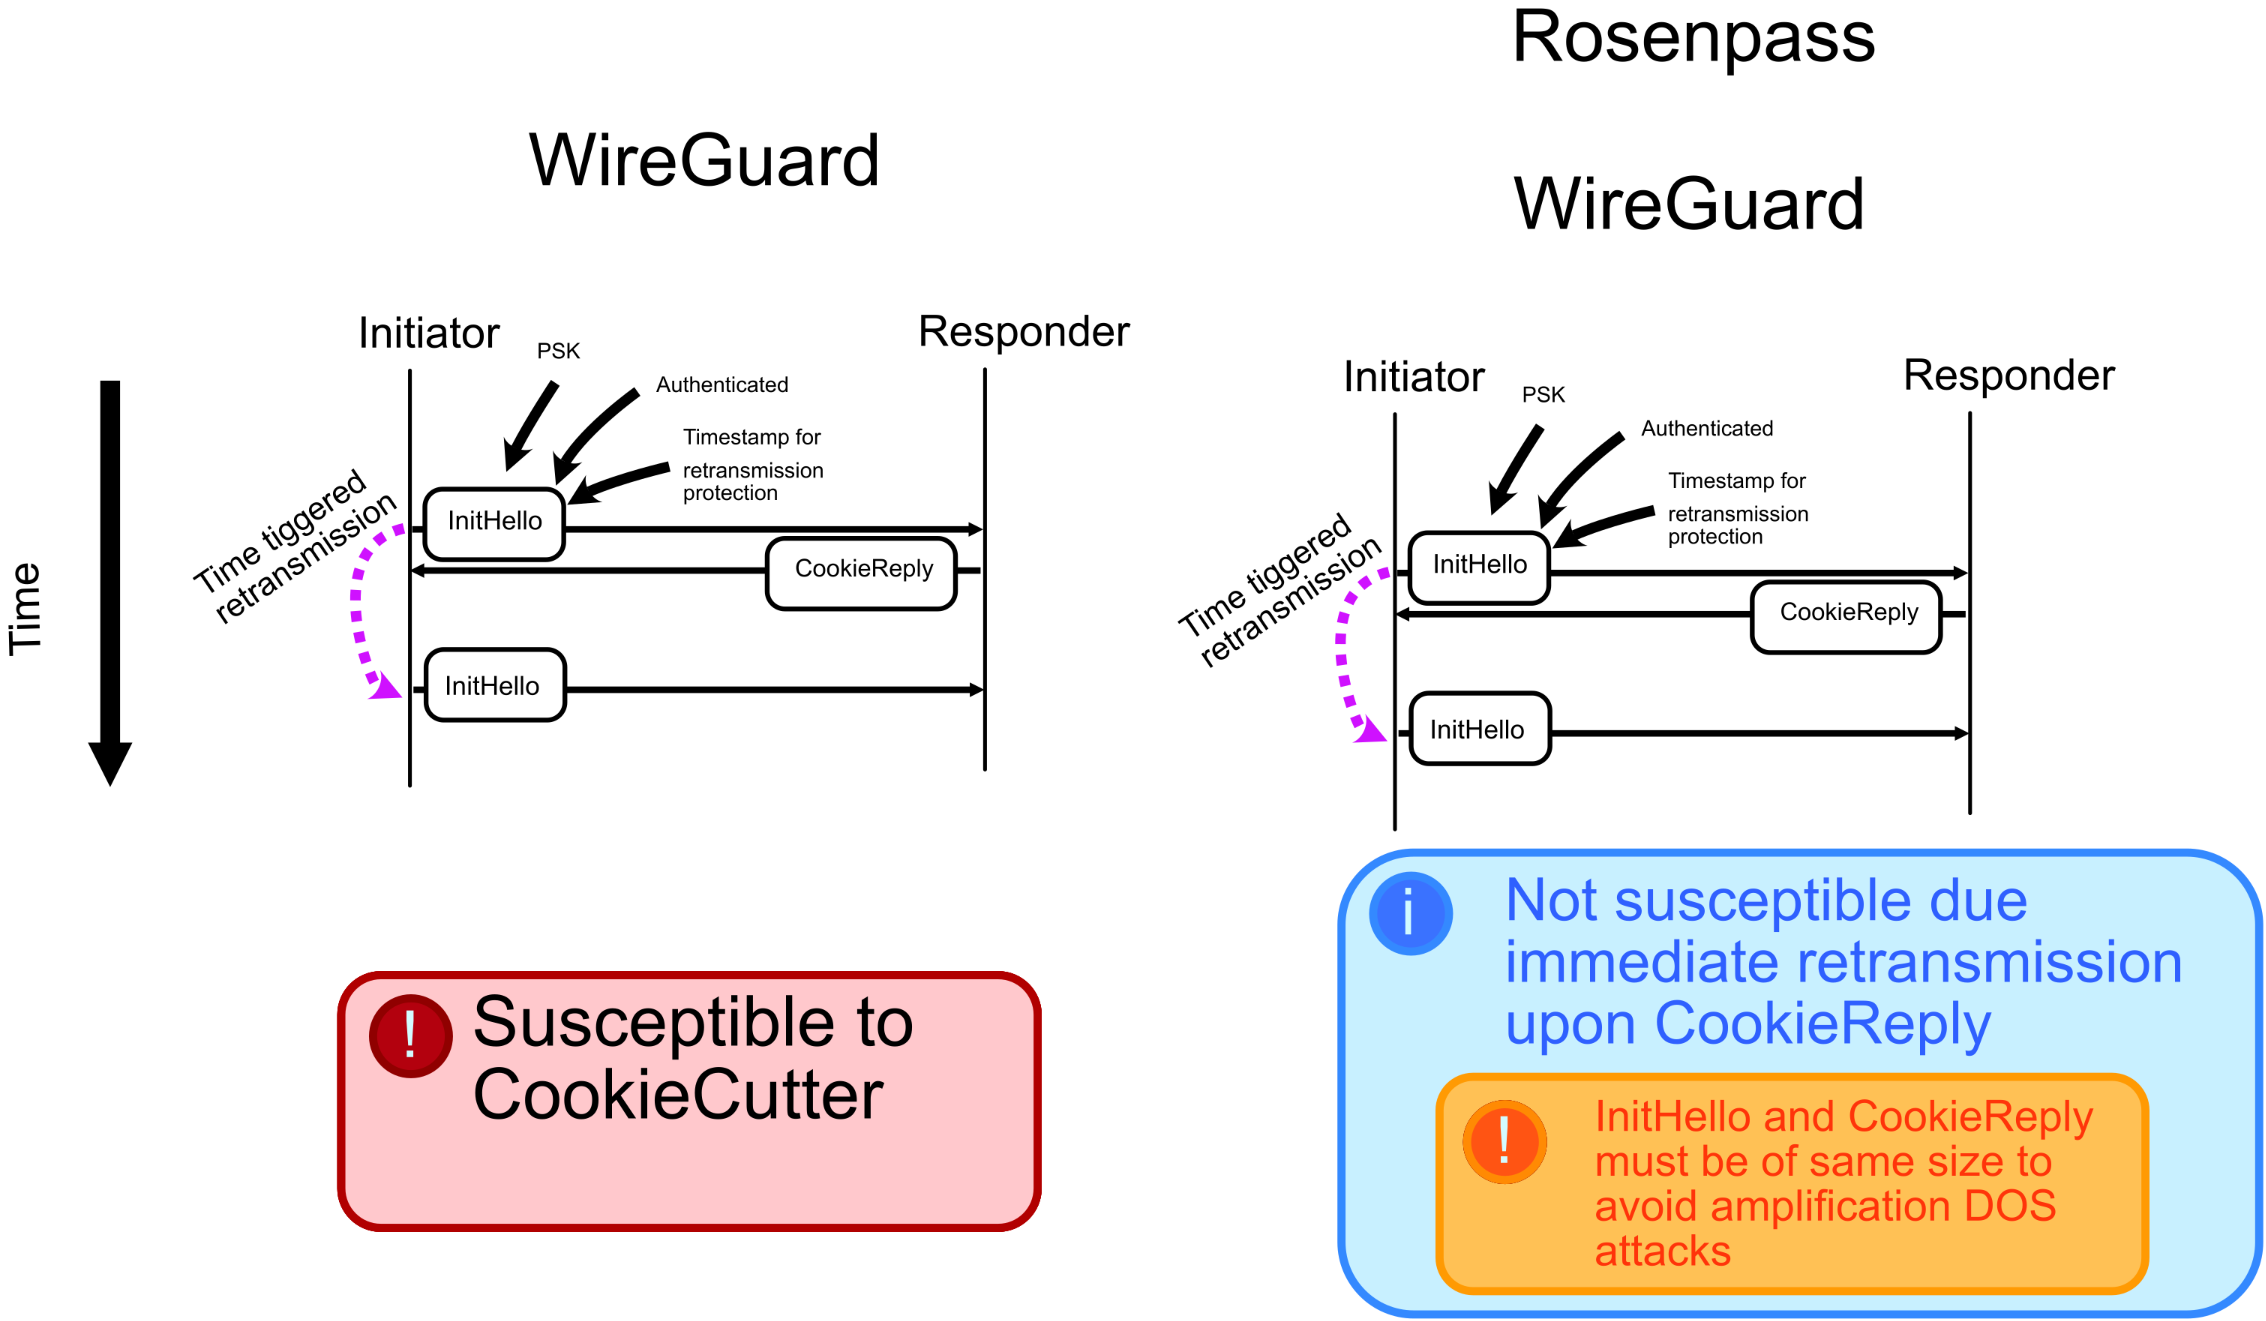
\includegraphics[keepaspectratio,width=.9\textwidth]{graphics/cookiecutter-compare.png}
%     \end{column}

%     \begin{column}{.6\textwidth}
%       \begin{itemize}
%       \item
%         WireGuard: Affected
%       \item
%         Post-Quantum WireGuard: Affected
%       \item
%         Rosenpass: Unaffected by immediate retransmission of InitHello upon
%         CookieReply receipt

%         \begin{itemize}
%         \item
%           (CookieReply and InitHello must be of same size)
%         \end{itemize}
%       \end{itemize}
%     \end{column}
%   \end{columns}
% \end{frame}

\interlude[4]<Trials \textasciitilde\ Advanced Security Properties>{Knock Patterns}

\begin{frame}{Rosenpass and WireGuard: Advanced Security}
\vspace*{-\baselineskip}
\small
\begin{columns}[fullwidth,T]
	\setlength\leftmargini{\labelwidth+\labelsep}
  \begin{column}{.48\linewidth}
% TODO(marei): Can we make the smilies look nicer
    \begin{block}{\strut CPU DoS mitigation:}
    \begin{itemize}
      \item No change on the protocol level.
      \item[{\Sey[][green!60!white]} ] Slightly worsened in practice because PQ operations are more expensive than elliptic curves
    \end{itemize}
        \unskip
    \end{block}
    \begin{block}{\strut Limited Stealth:}
    \begin{itemize}
      \item No change in Rosenpass, but we should have \textbf{full stealth}!
      \item[$\Rightarrow$] Remove cookie mechanism?
      \item[{\Sey[][green!60!white]} ] This would affect the CPU DoS mitigation too much.
    \end{itemize}
    \unskip
    \end{block}

  \end{column}

  \begin{column}{.48\linewidth}
    \begin{block}{\strut Limited Identity Hiding:}
    \begin{itemize}
      \item No change in Rosenpass, but we should have \textbf{full identity hiding}!
      \item[$\Rightarrow$] Do not use pre-authentication with public key?
      \item[{\Sey[][green!60!white]} ] This would affect the CPU DoS mitigation, possibly too much.
    \end{itemize}
        \unskip
    \end{block}
    % \textbf{Interruption resistance:} \vspace{0.5em} % TODO(blipp): Mark red somehow?
    % \begin{itemize}
    %   \item[ {\Laughey[1.4]} ] supported and modeled!
    % \end{itemize}
  \end{column}
\end{columns}
\end{frame}

% \begin{frame}{Rosenpass Advanced Security Properties}
% % :information\_source: (done) Insert protocol time diagram on left side

%   \begin{columns}[c]
%     \begin{column}{.4\textwidth}
%       \includegraphics[keepaspectratio,width=.9\textwidth]{rosenpass-whitepaper-key-exchange-protocol}
%     \end{column}

%     \begin{column}{.6\textwidth}
%       \only<1>{
%         \textbf{Limited Stealth:}

%         \begin{itemize}
%         \item
%           Protocol should not respond to packages without some
%           pre-authentication
%         \item
%           Proof of IP ownership (cookie mechanism) prevents full stealth
%         \item
%           Attacker needs to know responder key
%         \item
%           Full stealth needs initiator authentication in first package
%         \end{itemize}
%       }

%       \only<1-2>{
%         \textbf{Limited Identity Hiding:}

%         \begin{itemize}
%         \item
%           Attacker can guess identities due to use in the MAC in the auth code
%         \end{itemize}
%       }

%       \only<2-3>{
%         \textbf{Limited CPU DoS protection:}

%         \begin{itemize}
%         \item
%           Preventing CPU-exhaustion DoS involving network amplification
%           attacks
%         \item
%           Proof of IP ownership
%         \item
%           \textbf{Slightly more exposed due to more expensive cryptographic
%           operations}
%         \end{itemize}
%       }
%       
%       \only<3>{
%         \textbf{Full interruption (state disruption) resistance:} Stateless
%         responder

%         \textbf{Post-Quantum secure!}
%       }

%       \only<4>{
%       $\Rightarrow$
%         Rosenpass is as secure as WireGuard but using
%         PostQuantum security

%       $\Rightarrow$
%         Additional state disruption resistance

%       $\Rightarrow$
%         CPU-exhaustion resistance is slightly worse, but that
%         is due to the cost of the cryptographic primitives
%       }
%     \end{column}
%   \end{columns}
% \end{frame}

\begin{frame}{Choose Two: Stealth, Identity Hiding, CPU DoS Mit.}
  \centering
  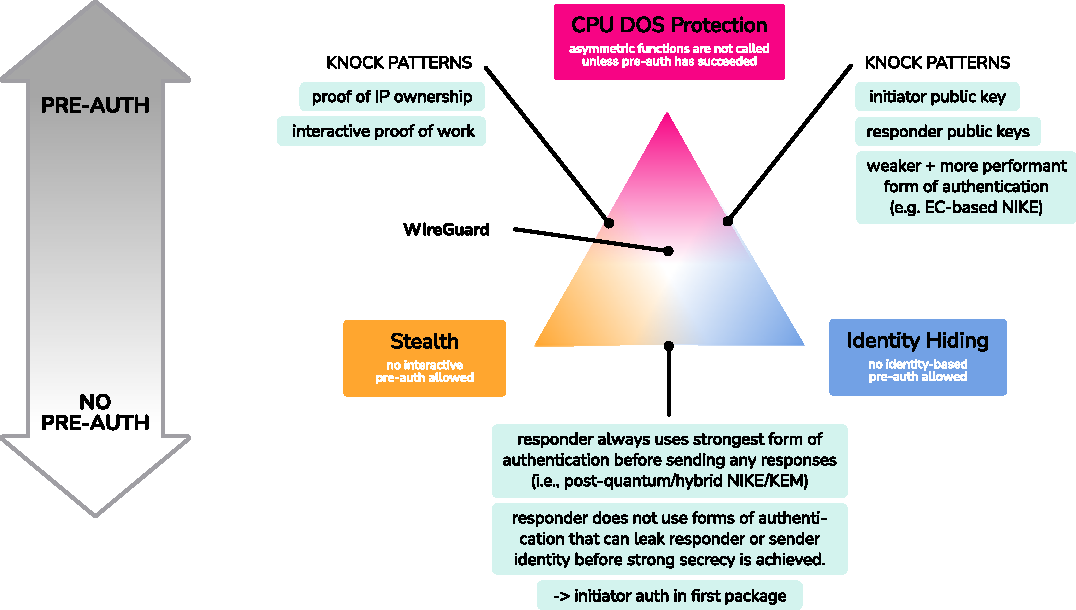
\includegraphics[height=.85\textheight]{graphics/preauth-tradeoff-bare.pdf}
\pdfpcnote{Stealth + Identity Hiding\\
* Disable pre-auth with public key in symmetric MAC\\
* Disable cookie-mechanism\\
* => No CPU DoS mitigation\\
\\
Stealth + CPU DoS mitig.\\
* Disable cookie-mechanism\\
* => Limited identity hiding due to public key in symmetric MAC\\
\\
Identity hiding + CPU DoS mitig.\\
* Disable pre-auth with public key in symmetric MAC\\
* => Limited stealth due to cookie mechanism
}
\end{frame}

%\begin{frame}{Choose Two: Stealth, Identity Hiding, CPU DoS Mit.}
%\begin{columns}[fullwidth,T]
%\begin{column}{.53\linewidth}
%\begin{overlayarea}{\linewidth}{ .85\textheight}
%\vfill
%\raisebox{-.5\height}{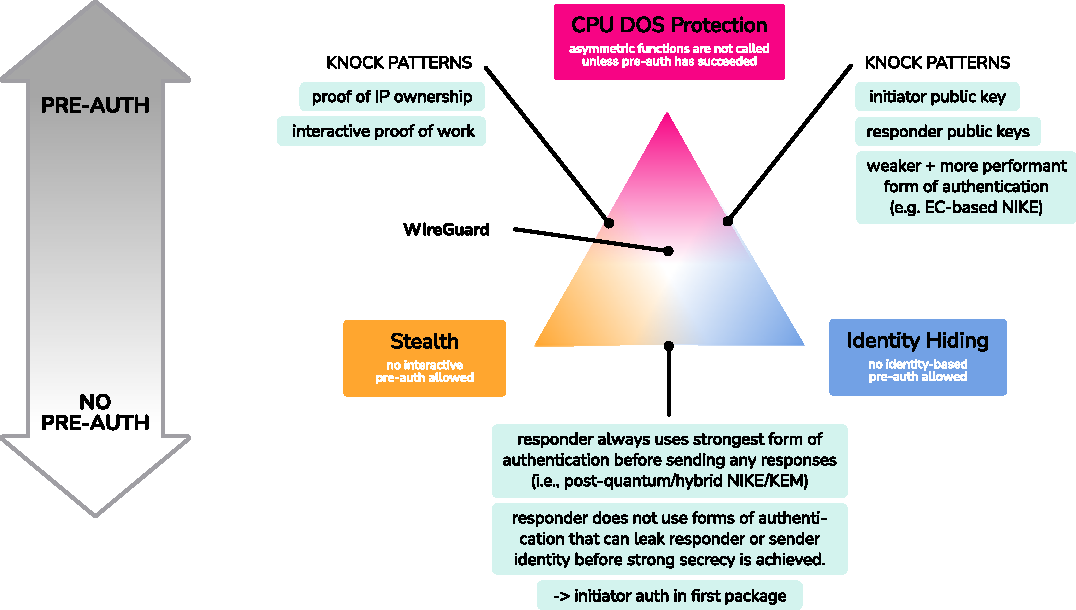
\includegraphics[width=\linewidth]{graphics/preauth-tradeoff-bare.pdf}}
%\par
%\vfill
%  \end{overlayarea}
%\end{column}%
%    \begin{column}{.45\linewidth}
%    \small
%      \begin{enumblock*}{Stealth + Identity Hiding:}
%      \only<+>{
%      \begin{itemize}
%        \item Disable pre-auth with public key in symmetric MAC
%        \item Disable cookie-mechanism
%        \item[$\Rightarrow$] No CPU DoS mitigation
%      \end{itemize}
%      \unskip}
%      \end{enumblock*}
%      \begin{enumblock*}{Stealth + CPU DoS mitig.:}
%      \only<+>{
%      \begin{itemize}
%        \item Disable cookie-mechanism
%        \item[$\Rightarrow$] Limited identity hiding due to public key in symmetric MAC
%      \end{itemize}
%      \unskip}
%      \end{enumblock*}
%      \begin{enumblock*}{Identity hiding + CPU DoS mitig.:}
%    \only<+>{
%      \begin{itemize}
%        \item Disable pre-auth with public key in symmetric MAC
%        \item[$\Rightarrow$] Limited stealth due to cookie mechanism
%      \end{itemize}
%      \unskip}
%      \end{enumblock*}
%    \end{column}
%\end{columns}
%\end{frame}

\begin{frame}{WireGuard and Rosenpass Trade-Offs}
  \begin{columns}[fullwidth,T]
\begin{column}{.53\linewidth}
\begin{overlayarea}{\linewidth}{ .85\textheight}
\vfill
\raisebox{-.5\height}{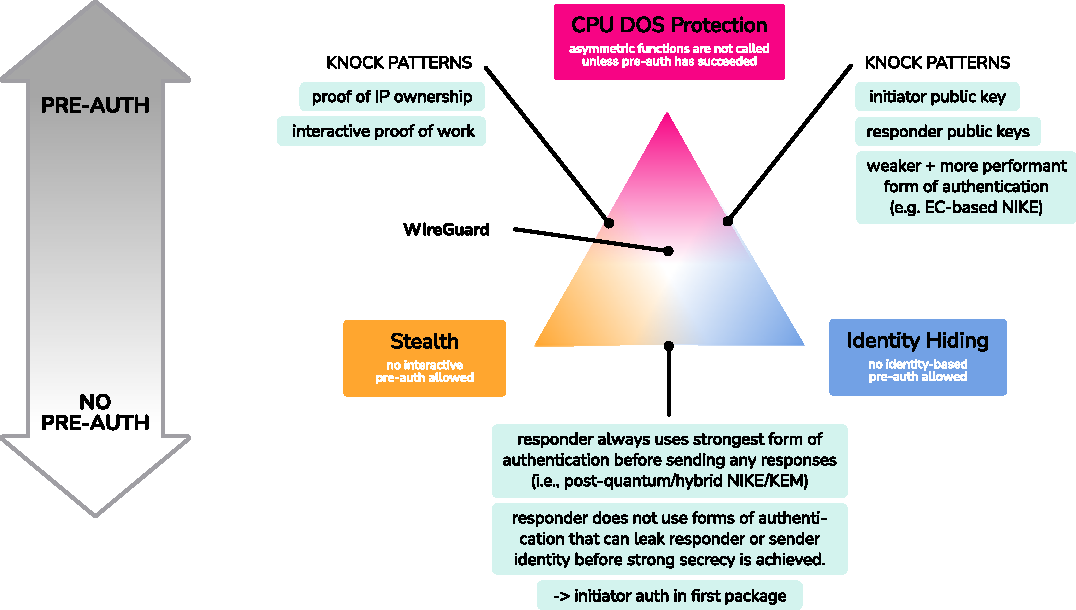
\includegraphics[width=\linewidth]{graphics/preauth-tradeoff-bare.pdf}}
\par
\vfill
\end{overlayarea}
\end{column}
    \begin{column}{.45\linewidth}
    \small
      \begin{block}{CPU DoS Mitigation:}
      \only<+|handout:+>{
      \begin{itemize}
        \item There is no clear optimum here.
        \item CPU DoS mitigation is never calling asymmetric crypto unless we know it succeeds (circular reasoning)
      \end{itemize}
      \unskip
      }
      \end{block}
       \begin{block}{Stealth:\vphantom{g}}
      \only<+|handout:+>{
      \begin{itemize}
        \item Broken on DoS attacks assuming recipient is known % TODO(blipp): Fact check
        \item[$\Rightarrow$] This seems acceptable
      \end{itemize}
      \unskip
      }
      \end{block}
    \begin{block}{Identity hiding:}
     \only<+|handout:+>{
      \begin{itemize}
        \item Broken on knowledge of public keys
        \item[$\Rightarrow$] This seems inacceptable!
        \item[$\Rightarrow$] Investigate proper identity hiding without overly impacting stealth and CPU DoS mitig.
      \end{itemize}
      \unskip
      }
      \end{block}
    \end{column}
  \end{columns}
\end{frame}

\begin{frame}{Knock Patterns}
\begin{columns}[fullwidth,c]
    \begin{column}{.45\linewidth}
    \rlap{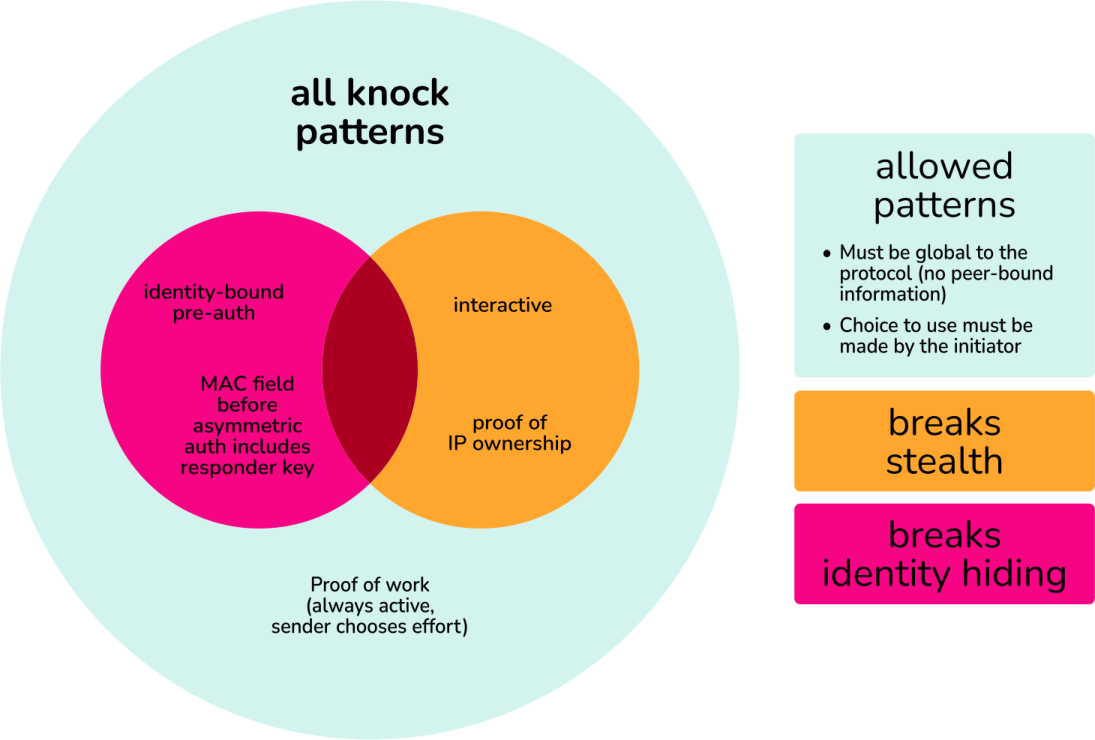
\includegraphics[keepaspectratio,width=\linewidth]{graphics/knock-patterns-bare.pdf}}
    \end{column}%
    \begin{column}{.5\linewidth}
      \begin{itemize}
        \item We choose to think of WireGuard's and Rosenpass' pre-auth as \say{Knock Patterns}
        \item These knock patterns have severe trade-offs.
        \item Interactive knock pattern (cookie mechanism) breaks stealth
        \item Identity-based knock patterns (e.g., knowledge of public key) breaks identity hiding
        \vspace{0.5em}
        \item[$\Rightarrow$] Avoid identity-bound knock patterns
        \item[$\Rightarrow$] Minimize interactive knock patterns
        \item[$\Rightarrow$] Explore other (allowed) knock patterns
      \end{itemize}
    \end{column}
  \end{columns}
\end{frame}


\begin{frame}{Tools to the Table!}
Bellare and Rogaway [BR06], Halevi [Hal05]:\\
\hspace{1.618em} Call for “automated tools, that can help write and verify game-based proofs”\\[1.618em]
%
\visible<2->{%
Do the tools \emph{actually help}? And if yes, whom?\\[1.618em]

ProVerif, Tamarin, CryptoVerif, EasyCrypt:\\
\hspace{1.618em} We like these tools, they are good!\\[1.618em]%
}
\visible<3->{%
They mostly help the \emph{formal verification experts} to:
\begin{itemize}
\item do analyses themselves, write papers
\item develop proof methodologies, foundation work for formal methods
\end{itemize}
}
% c.f. Manuel's talk about EasyCrypt
\end{frame}




%\begin{frame}{Pen and Paper proofs}
%
%% Karo talk:
%% * proof should be part of the engineering effort
%% * updating a pen-and-paper proof is a mess
%
%
%% the reasons from Joseph's talk, and
%% * pen-and-paper proofs are often read-only
%% * hard to maintain and update, especially so by other people
%% * part of engineering effort: gap to implemented systems too large?
%
%
%
%\begin{itemize}
%\item
%  Become increasingly unwieldy
%\item
%  Karolin anecdote: Recently found major issues in fairly prominent
%  paper, page N
%
%  \begin{itemize}
%  \item
%    (TODO: Handle issues found with Signal analysis)
%  \end{itemize}
%\item
%  Proof state is hard to keep track off
%\end{itemize}
%
%% :information\_source: Insert screen-shot of PostQuantum WireGuard
%% paper showing WireGuard proof differential
%\end{frame}
%
%% Issues with proof tools
%% ProVerif
%% * no syntax highlighting or other integration available in your favourite editor
%% * no good tooling for engineering at scale (e.g., macro language/preprocessor)
%% * hard to understand output and error messages
%
%
%
%
%
%\begin{frame}{ProVerif}
%% :information\_source: Insert screen-shot of our ProVerif analysis
%
%% :information\_source: Cut off screen-shot of our code
%
%
%% Karo talk
%% * no syntax highlighting in Vim
%% * preprocessor to be able to split up into multiple files
%% * educated guesswork with use of some tooling, but it is opaque/undocumented
%% * 
%
%% TODO
%% * add screenshot of raw output
%% * 
%
%
%\begin{itemize}
%\item
%  No syntax highlighting
%\item
%  No good tooling to do engineering at scale (karolin resorted to the C
%  preprocessor)
%\end{itemize}
%
%% :information\_source: Insert screen-shot of raw ProVerif output on
%% the left; out colorful output on the side. \textgreater{} Big letters
%% (text below) on white superimposed on split-screen screenshot
%
%ProVerif output is not made for Humans
%\end{frame}
%
%\begin{frame}{CryptoVerif}
%% :information\_source: Insert screen-shot of HPKE or WG analysis by
%% blipp
%
%% :information\_source: Cut off screen-shot
%
%TODO: Blipp - Expert driven engineering
%
%% :information\_source: Insert screen-shot of CV documentation saying
%% ``to be done''
%
%% :information\_source: Cut off screen-shot
%
%\begin{itemize}
%\item
%  Sometimes the information is simply lacking
%\item Automation focused
%\item Always operating on the entire proof state
%\item complete lack of tooling
%\end{itemize}
%
%% TODO screenshot CV manual “we will add some things here”
%% * screenshot game state, maybe HPKE
%
%
%\end{frame}
%
%\begin{frame}{Tamarin}
%% :information\_source: Insert screen-shot of horn clause in text
%
%\begin{itemize}
%\item
%  When we evaluated Tamarin for use in Rosenpass you had to directly
%  encode horn clauses
%\item
%  There are new frontends there now
%\item
%  This is the prover we know least about (looking for input!)
%\end{itemize}
%\end{frame}
%
%\begin{frame}{EasyCrypt}
%% :information\_source: Insert screen-shot of nice EC code
%
%\begin{itemize}
%\item
%  This appears to be the most complete approach right now
%\item
%  Writing proofs is hard
%\item
%  No demonstration of use with protocols at the moment
%\item
%  Anecdote:
%
%  \begin{itemize}
%  \item
%    When we tried out EC we asked advanced EC researchers at MPI-SP for
%    a tutorial to look at
%  \item
%    The tutorial contained an unknown syntax
%  \item
%    We where trying to figure out what this did
%  \item
%    I went to the very advanced researchers
%  \item
%    They thanked me for the interruption and started reverse engineering
%    the tool because they did not know either
%  \item
%    =\textgreater{} Engineering problem ``naturally-grown'' code bases
%  \end{itemize}
%\end{itemize}
%\end{frame}
%
%\begin{frame}{Protocol proof approaches}
%\begin{itemize}
%\item
%  Pen and paper proofs are hard to vet and error prone
%
%  \begin{itemize}
%  \item
%    Provide a lot of flexibility, this is a good thing
%  \end{itemize}
%\item
%  Formal verification tools work, but they are hard to use.
%
%  \begin{itemize}
%  \item
%    THEY ARE ALSO HARD TO READ EVEN FOR THE AUTHORS
%  \end{itemize}
%\item
%  Option: The basic models may be there
%
%  \begin{itemize}
%  \item
%    They are very strict and formally correct
%  \end{itemize}
%\item
%  We need more ability to hand-wave in formal methods proofs
%
%  \begin{itemize}
%  \item
%    This is supposed to make proofs easier; it is an incremental process
%  \end{itemize}
%\item
%  We need to improve tooling
%
%  \begin{itemize}
%  \item
%    More tooling (syntax highlighting, interactive proof assistants)
%  \item
%    More user experience (understandable output from proof verifcation
%    tools)
%  \item
%    More expressiveness
%  \end{itemize}
%\end{itemize}
%\end{frame}
%
%\begin{frame}{Protocol proof approaches}
%% :information\_source: Center text, no decorations (i.e.~no top bar),
%% big letters.
%
%More expressiveness in formal verification tools
%\end{frame}
%
%\begin{frame}{Oracle declarations in the Rosenpass ProVerif model}
%% :information\_source: Screen shot of one verbose oracle declaration
%in the Rosenpass symbolic model
%
%% :information\_source: Another screenshot
%
%% :information\_source: A screenshotg of a complex C macro in tghe
%% symbolic analysis
%
%% :information\_source: A screenshotg of a proverif macro expansion in
%% ProVerif
%
%% :information\_source: White text on the right side
%
%\begin{itemize}
%\item
%  A more powerful language with native support for complex syntax sugar
%  would help a lot
%\item
%  Syntax rewriting is a basic element of proofs
%\item
%  It is suprising that our cryptographic proof tools completely lack
%  support for native syntax extensions
%\item
%  Syntax rewriting is called ``macros'' when computer-scientists do it
%\item
%  We have a tool for that; it is called lisp
%\end{itemize}
%\end{frame}


\section{Section: Epilogue}

\interlude[6]{Epilogue}

% :information_source: Add wireGuard Dragon and Bunny
\setbeamertemplate{background canvas}{\vbox to .9\paperheight {\vspace*{\fill}\transparent{.1}\makebox[\paperwidth][c]{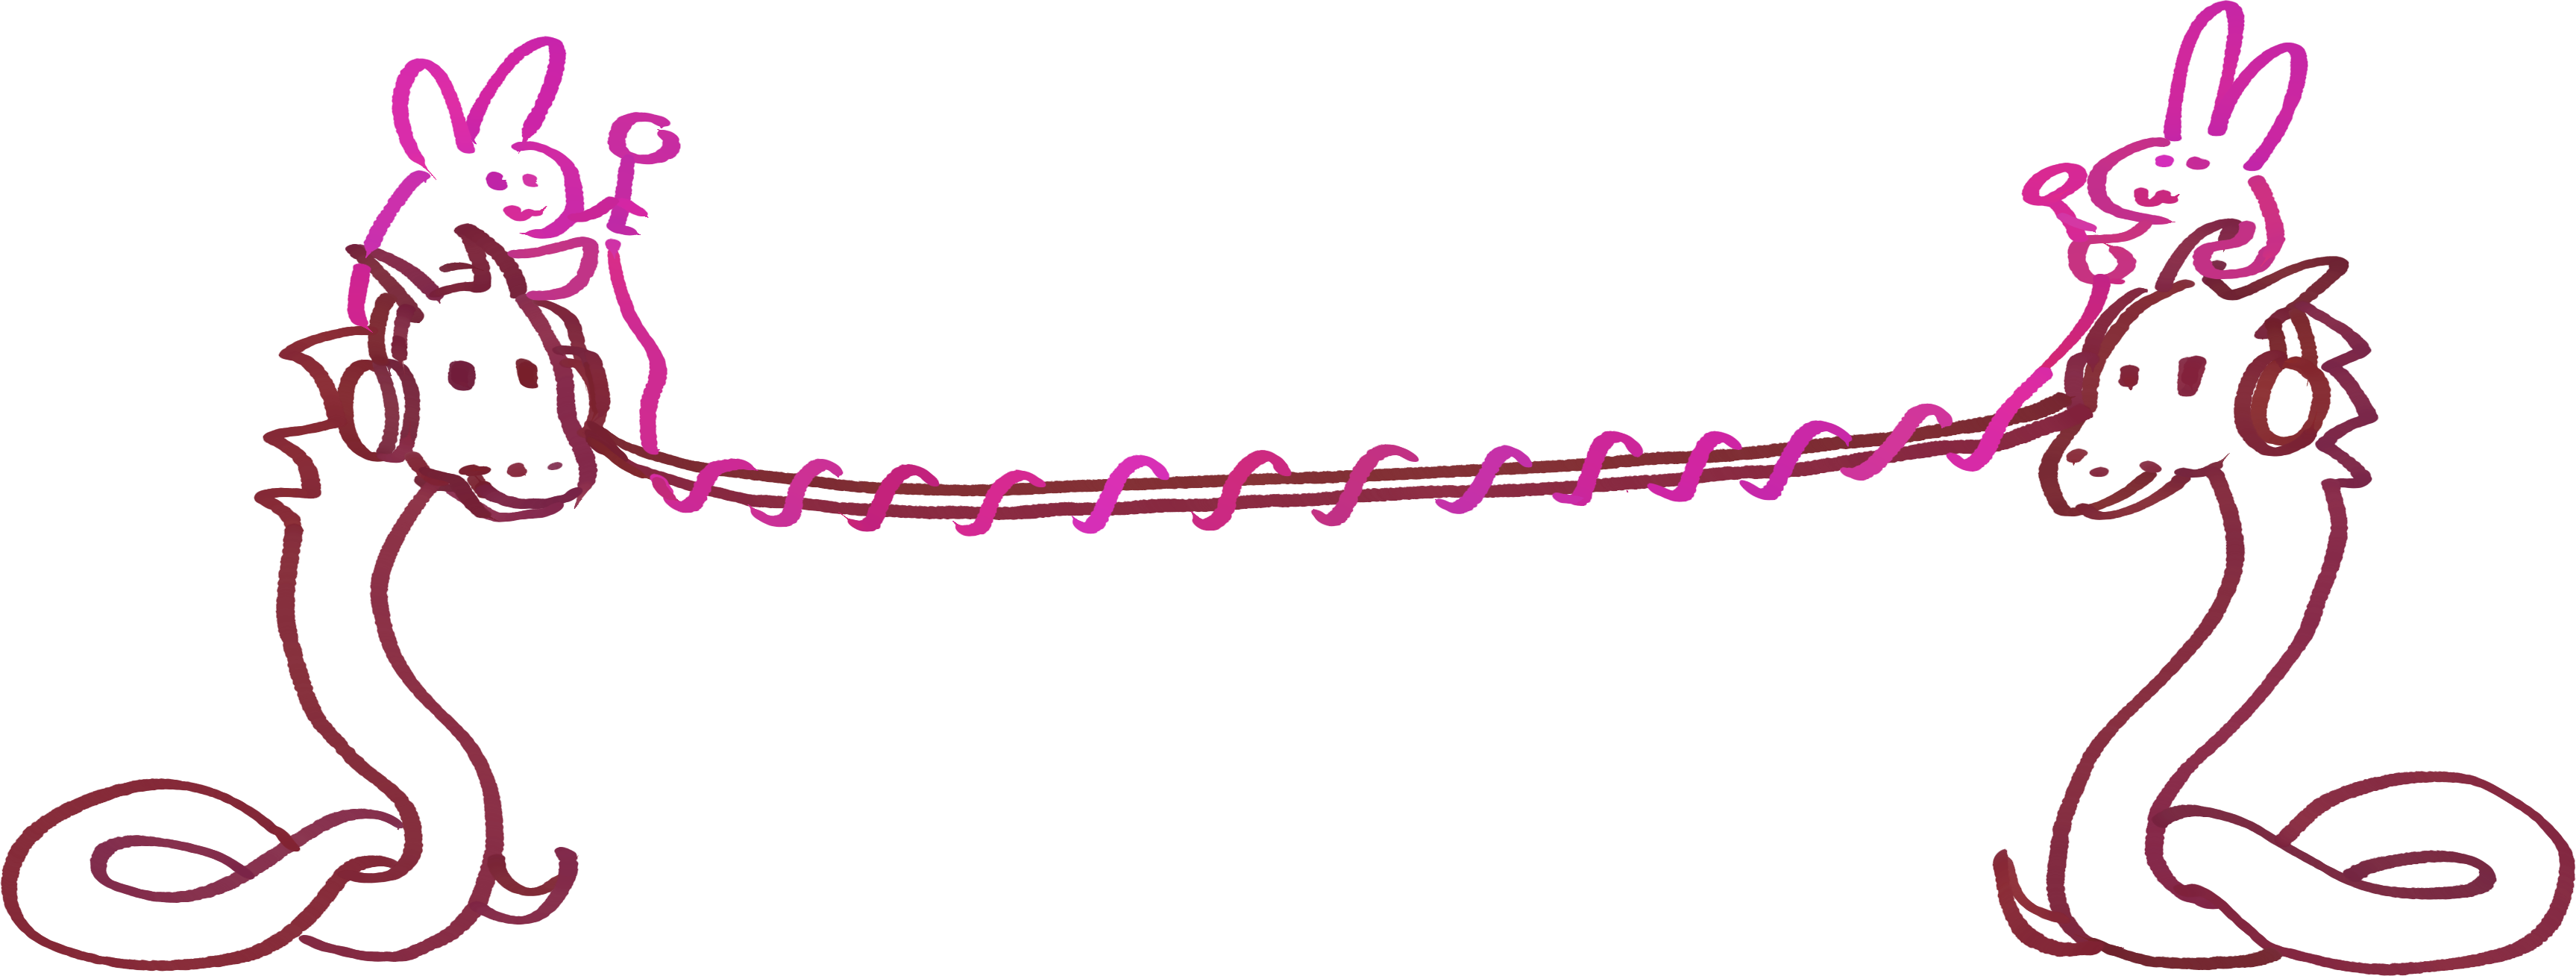
\includegraphics[width=\linewidth]{graphics/wireguard-and-rp-bunny-rose.png}}}}

\begin{frame}{Conclusion}
\vspace{-\ht\strutbox}
  \begin{columns}[t]
    \begin{column}{.30\linewidth}
      \begin{block}{Rosenpass\strut}
      \begin{itemize}
      \item
        Post-quantum secure AKE
      \item
        Same security as WireGuard
      \item
        Improved state disruption resistance
      \item
        Transfers key to WireGuard for hybrid security
      \end{itemize}
      \end{block}
    \end{column}

    \begin{column}{.33\linewidth}
      \begin{block}{Protocol Findings\strut}
      \begin{itemize}
      \item
        \textbf{CookieCutter}: DoS exploiting WireGuard cookie mechanism
      \item
        \textbf{ChronoTrigger}: DoS exploiting insecure system time to attack WireGuard
      \item
        There is a \textbf{trade-off} between identity hiding, stealth, and
        CPU-exhaustion DoS protection
      \end{itemize}
      \end{block}
    \end{column}

    \begin{column}{.36\linewidth}
      \begin{block}{Talk To Us\strut}
      \begin{itemize}
      \item
        About why we should use Tamarin (or SAPIC+?) over ProVerif
      \item
        State disruption attacks
      \item
        Stealth and Identity hiding
      \item
        Adding syntax rewriting to the tool belt of mechanized verification in
        cryptography
      \end{itemize}
      \vspace{2em}
      \hfill\textbf{\url{rosenpass.eu}}
      \end{block}
    \end{column}
  \end{columns}
\end{frame}


\begin{frame}{Rosenpass going Rube-Goldberg: The Details}
% :information\_source: Architecture diagram of python based proofs

% :information\_source: Scale graphic to allow for points
\small
\begin{itemize}
\item
  Embed cryptographic proof syntax in Lisp S-Expressions
\item
  Translate Lisp code to Python using the Hy language (Lisp that
  compiles to Python)
\item
  Translate S-Expression code to AST or DOM
\item
  Translate AST or DOM to ProVerif/Tamarin/CryptoVerif/EasyCrypt code using the
  LARK code parser/generator
\item
  Remote control ProVerif/Tamarin/CryptoVerif/EasyCrypt by

  \begin{itemize}
  \item
    Parsing their command line output using LARK
  \item
    (Possibly using the language server interface for more interactive
    features)
  \end{itemize}
\item
  Provide custom syntax using

  \begin{itemize}
  \item
    Lisp Macros
  \item
    Extending LARK-based syntax parsers (to add custom syntactic
    elements)
  \item
    AST Rewriting for more complex adaption
  \end{itemize}
\item
  Integrate with external tools by exporting our AST as XML

  \begin{itemize}
  \item
    XML is just a convenient grammar for trees
  \item
    We do not need to support the full complexity of XML including XML
    style sheets and such things
  \end{itemize}
\end{itemize}
\end{frame}
